% Chapter 14. Delegation shapes, and the failure each one isolates.
\documentclass[tikz,border=6pt]{standalone}
% Shared look for every TikZ figure in the book.
% Colours match book/preamble.tex exactly. Change both or neither.

\usepackage{tikz}
\usepackage{xcolor}
\usepackage{amsmath}
\IfFileExists{libertinus.sty}{\usepackage[mono=false]{libertinus}}{}
\IfFileExists{inconsolata.sty}{\usepackage[varqu,varl,scaled=0.95]{inconsolata}}{}

\usetikzlibrary{
  arrows.meta, positioning, calc, fit, backgrounds, shapes.geometric,
  shapes.misc, decorations.pathreplacing, decorations.pathmorphing,
  patterns, chains, matrix, shadows.blur
}

\definecolor{ink}{HTML}{15181D}
\definecolor{muted}{HTML}{5B6472}
\definecolor{rule}{HTML}{C9CED6}
\definecolor{wash}{HTML}{F4F5F7}
\definecolor{accent}{HTML}{0F5C8C}
\definecolor{accentsoft}{HTML}{E7F0F6}
\definecolor{warm}{HTML}{B4531A}
\definecolor{warmsoft}{HTML}{FBF0E7}
\definecolor{good}{HTML}{2C6E49}
\definecolor{goodsoft}{HTML}{E9F2EC}
\definecolor{danger}{HTML}{9B2226}
\definecolor{dangersoft}{HTML}{FAECEC}

\tikzset{
  font=\sffamily\small,
  >={Stealth[length=5pt, width=4pt]},
  %
  box/.style={
    draw=rule, line width=0.8pt, fill=wash, rounded corners=2pt,
    inner sep=7pt, align=center, text=ink, minimum height=9mm,
  },
  boxa/.style={box, draw=accent, fill=accentsoft},
  boxg/.style={box, draw=good,   fill=goodsoft},
  boxw/.style={box, draw=warm,   fill=warmsoft},
  boxd/.style={box, draw=danger, fill=dangersoft},
  %
  lane/.style={draw=rule, line width=0.7pt, fill=white, rounded corners=2pt,
               inner sep=6pt, align=center, minimum width=26mm},
  %
  flow/.style={draw=accent, line width=1.0pt, ->},
  flowback/.style={flow, densely dashed},
  flowmuted/.style={draw=muted, line width=0.8pt, ->},
  lifeline/.style={draw=rule, line width=0.7pt, densely dotted},
  %
  lbl/.style={font=\sffamily\scriptsize, text=muted, inner sep=2pt},
  lblink/.style={font=\sffamily\scriptsize, text=ink, inner sep=2pt},
  tag/.style={font=\ttfamily\scriptsize, text=accent, inner sep=2pt,
              fill=white, inner xsep=3pt},
  note/.style={font=\sffamily\scriptsize\itshape, text=muted, align=left},
  %
  band/.style={draw=none, rounded corners=1pt},
  tick/.style={draw=muted, line width=0.6pt},
}

% A horizontal timeline bar segment: \barseg{x0}{x1}{y}{colour}{label}
\newcommand{\barseg}[5]{%
  \fill[#4, rounded corners=1pt] (#1,#3-0.16) rectangle (#2,#3+0.16);
  \node[lbl, text=white, font=\sffamily\scriptsize\bfseries]
       at ({(#1+#2)/2},#3) {#5};
}

\begin{document}
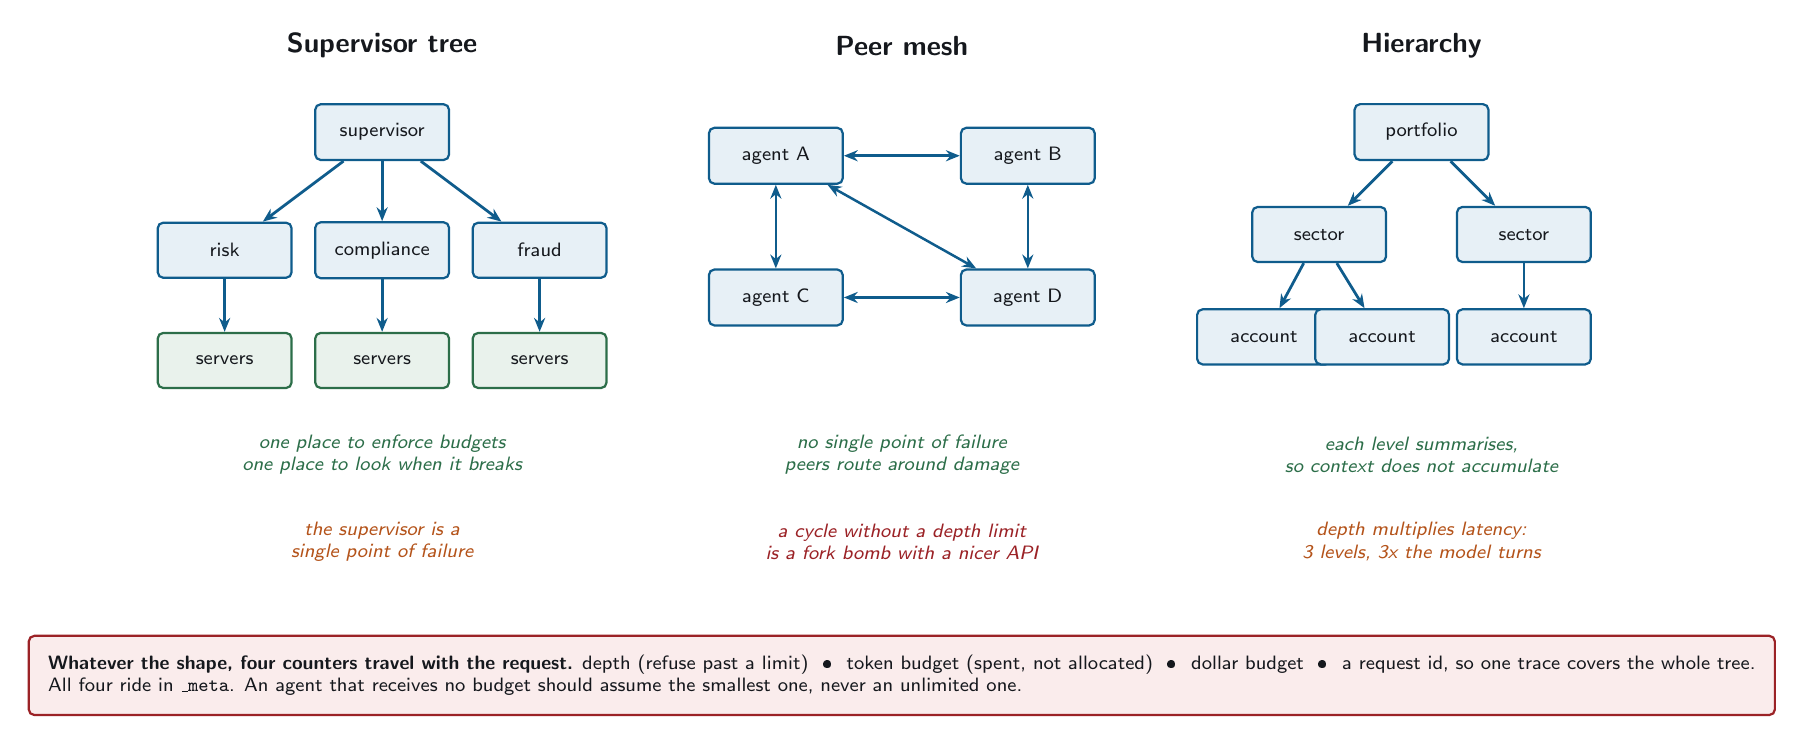
\begin{tikzpicture}[x=1cm, y=1cm]

\tikzset{ag/.style={boxa, minimum width=17mm, minimum height=7mm,
                    font=\sffamily\scriptsize},
          sv/.style={boxg, minimum width=17mm, minimum height=7mm,
                    font=\sffamily\scriptsize}}

% ------------------------------------------------------------- supervisor
\begin{scope}[xshift=0cm]
  \node[lblink, font=\sffamily\bfseries] at (2.0,3.6) {Supervisor tree};

  \node[ag] (sup) at (2.0,2.5) {supervisor};
  \node[ag] (r) at (0.0,1.0) {risk};
  \node[ag] (c) at (2.0,1.0) {compliance};
  \node[ag] (f) at (4.0,1.0) {fraud};
  \node[sv] (s1) at (0.0,-0.4) {servers};
  \node[sv] (s2) at (2.0,-0.4) {servers};
  \node[sv] (s3) at (4.0,-0.4) {servers};

  \foreach \x in {r,c,f} { \draw[flow] (sup) -- (\x); }
  \draw[flow] (r) -- (s1); \draw[flow] (c) -- (s2); \draw[flow] (f) -- (s3);

  \node[note, align=center, text=good] at (2.0,-1.6)
    {one place to enforce budgets\\one place to look when it breaks};
  \node[note, align=center, text=warm] at (2.0,-2.7)
    {the supervisor is a\\single point of failure};
\end{scope}

% ------------------------------------------------------------------- mesh
\begin{scope}[xshift=6.6cm]
  \node[lblink, font=\sffamily\bfseries] at (2.0,3.6) {Peer mesh};

  \node[ag] (a) at (0.4,2.2) {agent A};
  \node[ag] (b) at (3.6,2.2) {agent B};
  \node[ag] (d) at (0.4,0.4) {agent C};
  \node[ag] (e) at (3.6,0.4) {agent D};

  \draw[<->, draw=accent, line width=0.9pt] (a) -- (b);
  \draw[<->, draw=accent, line width=0.9pt] (a) -- (d);
  \draw[<->, draw=accent, line width=0.9pt] (b) -- (e);
  \draw[<->, draw=accent, line width=0.9pt] (d) -- (e);
  \draw[<->, draw=accent, line width=0.9pt] (a) -- (e);

  \node[note, align=center, text=good] at (2.0,-1.6)
    {no single point of failure\\peers route around damage};
  \node[note, align=center, text=danger] at (2.0,-2.7)
    {a cycle without a depth limit\\is a fork bomb with a nicer API};
\end{scope}

% -------------------------------------------------------------- hierarchy
\begin{scope}[xshift=13.2cm]
  \node[lblink, font=\sffamily\bfseries] at (2.0,3.6) {Hierarchy};

  \node[ag] (top) at (2.0,2.5) {portfolio};
  \node[ag] (m1) at (0.7,1.2) {sector};
  \node[ag] (m2) at (3.3,1.2) {sector};
  \node[ag] (l1) at (0.0,-0.1) {account};
  \node[ag] (l2) at (1.5,-0.1) {account};
  \node[ag] (l3) at (3.3,-0.1) {account};

  \draw[flow] (top) -- (m1); \draw[flow] (top) -- (m2);
  \draw[flow] (m1) -- (l1); \draw[flow] (m1) -- (l2);
  \draw[flow] (m2) -- (l3);

  \node[note, align=center, text=good] at (2.0,-1.6)
    {each level summarises,\\so context does not accumulate};
  \node[note, align=center, text=warm] at (2.0,-2.7)
    {depth multiplies latency:\\3 levels, 3x the model turns};
\end{scope}

% ------------------------------------------------------------------ rules
\node[boxd, minimum width=178mm, align=left, font=\sffamily\scriptsize]
  at (8.6,-4.4)
  {\textbf{Whatever the shape, four counters travel with the request.}
   depth (refuse past a limit) \ \textbullet\ \
   token budget (spent, not allocated) \ \textbullet\ \
   dollar budget \ \textbullet\ \
   a request id, so one trace covers the whole tree.\\
   All four ride in \texttt{\_meta}. An agent that receives no budget should
   assume the smallest one, never an unlimited one.};

\end{tikzpicture}
\end{document}
